\chapter{Геометрические вероятности}

\section*{Введение}

Геометрическое определение вероятности является обощение классического определения на случай несчетных множеств элементарных исходов $\Omega$. Предполагается наличие некоторой
"геометрической"{} меры $\mu$, определенной для всех событий $A \in S$ алгебры событий $S$ (в том числе и для $\Omega \in S$). С помощью меры $\mu$ вводится вероятностная мера
$P$:
\begin{equation}
    P \left ( A \right ) = \frac{\mu \left ( A \right )}{\mu \left ( \Omega \right )}.
\end{equation}

Как правило, в качестве меры $\mu$ на практике выступает понятия длины, площади, объёма.

\section*{Задача 18.140}

Внутри квадрата с вершинами (0, 0), (1, 0), (1, 1) и (0, 1) наудачу выбирается точка $M(x,y)$. Найти вероятность события $B = \event{(x, y) | xy < a, a > 0}$.

\subsection*{Решение:}

В данном случае множество всех элементарных исходов представляет собой точки квадрата:
\begin{equation}
    \Omega = \left \{ (x, y) : 0 \le x, y \le 1 \right \}.
\end{equation}

В качестве "геометрической"{} меры $\mu$ используется площадь, поэтому
\begin{equation}
    \mu \left ( \Omega \right ) = 1.
\end{equation}

Форма события $B$ зависит от значения параметра $a$.
\begin{enumerate}
    \item
    Если $a > 1$, то все точки $(x,y)$ квадрата $\Omega$ удовлетворяют условию $x y < a$, поэтому
    \begin{equation}
        B = \Omega,
    \end{equation}
    и вероятность события $B$:
    \begin{equation}
        \probability{B}
        = \frac{\mu \left ( B \right )}{\mu \left ( \Omega \right )}
        = \frac{\mu \left ( \Omega \right )}{\mu \left ( \Omega \right )}
        = 1 .
    \end{equation}

    \item
    Если $0 < a \le 1$, тогда множество точек $B$ можно представить в виде объединения двух непересекающихся множеств (рисунок \ref{figure:lesson_3:40:B}):
    \begin{equation}
        B = B_1 + B_2 ,
    \end{equation}
    где $B_1$ --- прямоугольное множество и $B_2$ --- множество точек под гиперболой.

    \begin{figure}[h]
        \centering
        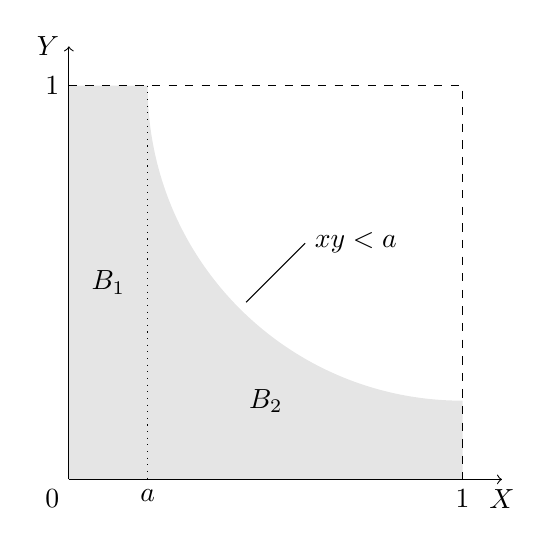
\begin{tikzpicture}[scale=5]
            \def \a {0.2};
            % фигура события
            \path [fill=gray!20] ( 0, 0 ) -- ( 0, 1 ) -- ( \a, 1 ) to [out=-90,in=180] ( 1, \a ) -- ( 1, 0 ) -- ( 0, 0 );
            \draw ( 0.45, 0.45 ) -- ( 0.6, 0.6 ) node [right] ( 0.6, 0.6 ) {$xy < a$};

            % оси
            \draw [->] ( 0, 0 ) -- ( 1.1, 0 ) node [below] at ( 1.1, 0 ) {$X$};
            \draw [->] ( 0, 0 ) -- ( 0, 1.1 ) node [left] at ( 0, 1.1 ) {$Y$};
            \node [below left] at ( 0, 0 ) {$0$};
            \node [below] at ( 1, 0 ) {$1$};
            \node [left] at ( 0, 1 ) {$1$};

            % границы квадрата
            \draw [dashed] ( 0, 1 ) -- ( 1, 1 ) -- ( 1, 0 );
            \draw [dotted] ( \a, 1 ) -- ( \a, 0 ) node [below] at ( \a, 0 ) {$a$};
            \node at ( 0.1, 0.5) {$B_1$};
            \node at ( 0.5, 0.2) {$B_2$};
        \end{tikzpicture}
        \caption{Событие $B = B_1 + B_2$.}
        \label{figure:lesson_3:40:B}
    \end{figure}

    Мера множества $B_1$ легко вычисляется --- это площадь прямоугольника:
    \begin{equation}
        \mu \left ( B_1 \right )
        = 1 \cdot a
        = a .
    \end{equation}

    Мера множества $B_2$ --- площадь под гиперболой $y = \frac{a}{x}$:
    \begin{equation}
        \mu \left ( B_2 \right )
        = \int \limits_{a}^1 \frac{a}{x} dx
        = \left . a \ln x \right |_a^1
        = a \left ( \ln 1 - \ln a \right )
        = - a \ln a .
    \end{equation}

    Вероятность события $B$:
    \begin{equation}
        \probability{B}
        = \frac{\mu \left ( B \right )}{\mu \left ( \Omega \right )}
        = \frac{\mu \left ( B_1 + B_2 \right )}{\mu \left ( \Omega \right )}
        = \frac{\mu \left ( B_1 \right ) + \mu \left ( B_2 \right )}{\mu \left ( \Omega \right )}
        = \frac{a - a \ln a}{1}
        = a \left ( 1 - \ln a \right ).
    \end{equation}
\end{enumerate}

\subsection*{Ответ:}
$
\probability{B} =
\left \{
\begin{array}{ll}
    a \left ( 1 - \ln a \right ), & 0 < a \le 1 \\
    1,         & 1 < a
\end{array}
\right .
.
$